
        % Ve nut ket thuc
        plot((xmin+xmax)/2,ymin,'ob');
        hold off
        
        % Chen cac 
        title('Graph of the clique Singletons')
        axis([xmin xmax ymin ymax+1])
        
        % Ve he truc hoac khong
        if c==0
            axis off
        else
            grid
        end % if c==0
        figure(1)

end % for function
    \end{lstlisting}
\end{lstlisting}

\begin{dl}
 Nội dung định lý viết vào đây   
\end{dl}

\cm{
Nội dung CM viết vào đây.
}

\begin{tc}
    
\end{tc}

\begin{md}
    
\end{md}

\begin{cy}
    
\end{cy}

\begin{vd}
    
\end{vd}

\begin{nx}
    
\end{nx}

\begin{bd}
    
\end{bd}

\subsection{Tiểu mục 2}
\begin{figure}[h!]
    \centering
    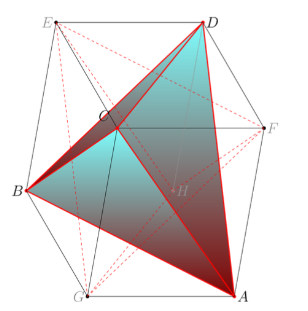
\includegraphics[width=0.3\linewidth]{../../assets/images/figure-1.png}
    \caption{Hình minh họa 1}
    \label{fig:enter-label}
\end{figure}

% nội dung này có thể tham khảo giáo trình ĐSTT và HH2
\section{Mục 2}
\subsection{Tiểu mục 1}

\subsection{Tiểu mục 2}
\chapter{Phân tích nhiều chiều dữ liệu thang đo định lượng}

Nội dung này được tham khảo và tổng hợp từ các tài liệu tham khảo  .....

\section{Kiem dinh Pearson}
\subsection{Ham phan phoi tich luy}
\begin{equation}
    F(x) = P(X<x)
\end{equation}

% Mỗi hình một caption
\begin{figure}[h]
    \centering
    % Hình thứ nhất
    \begin{minipage}{0.45\textwidth}
        \centering
        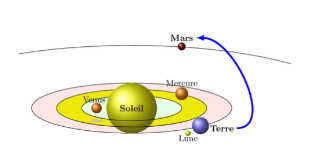
\includegraphics[width=\textwidth]{../../assets/images/figure-2.png}
        \caption{Hình 1}
        \label{fig:image1}
    \end{minipage}
    \hfill
    % Hình thứ hai
    \begin{minipage}{0.45\textwidth}
        \centering
        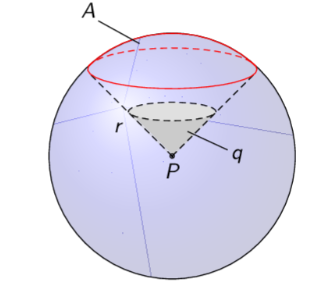
\includegraphics[width=0.7\textwidth]{../../assets/images/figure-3.png}
        \caption{Hình 2}
        \label{fig:image2}
    \end{minipage}
\end{figure}

% Hai hình 1 caption
\begin{figure}[h]
    \centering
    % Hình thứ nhất
